\scanpage{64}
de sorte qu'on aura \deleted{compatibilité} \inserted{commutativité} de
\diagram{\begin{tikzcd}[ampersand replacement=\&,column sep=large,row sep=large]
\&\Pi_{03}\arrow[dl,"\Psi_i^\omega"',"\deleted{\Pi_{03}}"]\arrow[d,"\psi_i^{\omega\deleted{\unsure{\varepsilon}}}"]\arrow[dr,"\psi_\omega^i"]\&\\
(44)\quad\Pi_{\unsure{0|1}}(\widetilde\Sigma,R_{\omega i}^\omega)\&\begin{array}{c}\Pi_1(\widetilde\Sigma,Q_i)\\=\Pi_i\end{array}\arrow[l,"b_i^{\omega'}(\cdot)"',"{\deleted{\unsure{\rightarrow}}}"{description,pos=.08}]\&\begin{array}{c}\Pi_1(\widetilde\Sigma,P_\omega)\\=\Pi_\omega\end{array}\arrow[l,"\varphi_{i\omega}=c_i^\omega(\cdot)"',"{\deleted{\unsure{\rightarrow}}}"{description,pos=.08}]
\end{tikzcd}}
où on a écrit $P_\omega$ au lieu de $P_\varepsilon$ (en identifiant $\uline{\omega}$ et $\uline{\varepsilon}$ grâce à $\unsure{\bar\omega|\varpi}_+$) et $\psi_i^\omega$ au lieu de $\psi_i^{\omega,\omega}$, $\psi_\omega^i$ au lieu de $\psi_\omega^{i,\omega}$.

Le passage à expliciter est celui de
\diagram{\begin{tikzcd}[ampersand replacement=\&,column sep=large]
\deleted{R_{\omega i}}\Pi_i^\omega\simeq\Pi_1(\widetilde\Sigma,R_{\omega i}^{\omega})\&\text{à}\&\Pi_i^{\omega'}=\Pi_1(\widetilde\Sigma,R_{\omega'i}^{\omega'})\\
\Pi_{0,3}\arrow[u,"\psi_i^\omega","\sim"']\&\&\Pi_{03}\arrow[u,"\psi_i^{\omega'}","\sim"']
\end{tikzcd}}
\inserted{Via $\widetilde b_{i\omega}$.}
\figure{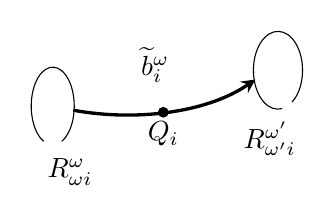
\begin{tikzpicture}[scale=1.3,>=stealth]
\draw(-.089,-.344)arc[start angle=245,end angle=-65,x radius=.21,y radius=.38];\draw(2.242,-.024)arc[start angle=280,end angle=-55,x radius=.24,y radius=.38];
\draw[->,very thick](.2,-.04)..controls(.8,-.15)and(1.5,-.07)..(1.98,.26);
\fill(1.08,-.06)circle(1.5pt)node[below]{$Q_i$};\node at(1,.4){$\widetilde b_i^\omega$};
\node[below]at(.17,-.42){$R_{\omega i}^{\omega}$};\node[below]at(2.12,-.06){$R_{\omega'i}^{\omega'}$};
\end{tikzpicture}}
On trouve par la commutativité (44) et par la dernière formule (39) qu'on a
\deleted{$\unsure{\widetilde b_{\omega\omega'}}$}
\[
(45)\qquad\widetilde b_i^\omega\bigl(\psi_i^\omega(\deleted{\unsure{g}}x)\bigr)=\psi_i^{\omega'}\bigl(\sigma_\infty(x)\bigr).
\]
\margin{63}
